%%%%%%%%%%%%%%%%%%%%%%%%%%%%%%%%%%%%%%%%%%%%%%%%%%%%%%
% A Beamer template for University of Wollongong     %
% Based on THU beamer theme                          %
% Author: Qiuyu Lu                                   %
% Date: July 2024                                    %
% LPPL Licensed.                                     %
%%%%%%%%%%%%%%%%%%%%%%%%%%%%%%%%%%%%%%%%%%%%%%%%%%%%%%
% Customized for Sharif University of Technology     %
%%%%%%%%%%%%%%%%%%%%%%%%%%%%%%%%%%%%%%%%%%%%%%%%%%%%%%


\documentclass[serif, aspectratio=169]{beamer}
%\documentclass[serif]{beamer}  % for 4:3 ratio
\usepackage[T1]{fontenc} 
\usepackage{fourier} % see "http://faq.ktug.org/wiki/uploads/MathFonts.pdf" for other options
\usepackage{hyperref}
\usepackage{latexsym,amsmath,xcolor,multicol,booktabs,calligra}
\usepackage{graphicx,pstricks,listings,stackengine}
\usepackage{lipsum}
\usepackage{tikz}

\usepackage{caption}
\usepackage{multirow}
\usepackage{array}
\usepackage{ragged2e}

\author{Ali Sharifi-Zarchi}
% \author{CE Department}
\title{Machine Learning (CE 40477)}
\subtitle{Fall 2024}
\institute{
    CE Department \\
    Sharif University of Technology
}
%\date{\small \today}
% \usepackage{UoWstyle}
\usepackage{SUTstyle}

% defs
\def\cmd#1{\texttt{\color{red}\footnotesize $\backslash$#1}}
\def\env#1{\texttt{\color{blue}\footnotesize #1}}
\definecolor{deepblue}{rgb}{0,0,0.5}
\definecolor{deepred}{RGB}{153,0,0}
\definecolor{deepgreen}{rgb}{0,0.5,0}
\definecolor{halfgray}{gray}{0.55}

\lstset{
    basicstyle=\ttfamily\small,
    keywordstyle=\bfseries\color{deepblue},
    emphstyle=\ttfamily\color{deepred},    % Custom highlighting style
    stringstyle=\color{deepgreen},
    numbers=left,
    numberstyle=\small\color{halfgray},
    rulesepcolor=\color{red!20!green!20!blue!20},
    frame=shadowbox,
}

\begin{document}

\begin{frame}
    \titlepage
    \vspace*{-0.6cm}
    \begin{figure}[htpb]
        \begin{center}
            
\includegraphics[keepaspectratio, scale=0.25]{pic/sharif-main-logo.png}
        \end{center}
    \end{figure}
\end{frame}

\begin{frame}    
\tableofcontents[sectionstyle=show,
subsectionstyle=show/shaded/hide,
subsubsectionstyle=show/shaded/hide]
\end{frame}

\section{Overview}
\begin{frame}{Parametric vs. non-parametric methods}
    \begin{itemize}
        \item \textbf{Parametric} methods need to \textbf{find parameters} from data and then use the inferred parameters to decide on new data points
        \begin{itemize}
            \item Learning: finding parameters from data
            \item e.g., \textbf{Linear regression}, \textbf{Logistic regression}
        \end{itemize}
        \item \textbf{Non-parametric} methods
        \begin{itemize}
            \item Training examples are \textbf{explicitly} used
            \item \textbf{Training phase} is \textbf{not required}
            \item e.g., \textbf{k-Nearest neighbors (kNN)}
        \end{itemize}
        \item Both supervised and unsupervised learning can be categorized into parametric and non-parametric methods
    \end{itemize}
\end{frame}
%%%%%%%%%%%%%%%%%%%%%%%%%%%%%%%%%%%%%%%%
\begin{frame}{Non-parametric learners}
    \begin{itemize}
        \item \textbf{Memory-based} or \textbf{Instance-based} learners
        \begin{itemize}
            \item lazy learning: (almost) all the work at the test time
        \end{itemize}
        
        \item Generic description:
        \begin{itemize}
            \item Memorize training $(x^{(1)}, y^{(1)}), \dots, (x^{(n)}, y^{(n)})$
            \item Given test $x$ predict: $\hat{y} = f(x;x^{(1)}, y^{(1)}, \dots, x^{(n)}, y^{(n)})$
        \end{itemize}
        \item $f$ is typically expressed in terms of the similarity of the test samples $x$ to the training samples $x^{(1)}, \dots, x^{(n)}$
        \item kNN is an instance-based learner
    \end{itemize}
\end{frame}

\section{k-Nearest-Neighbor}
    
\begin{frame}{kNN concept}
    \begin{figure}[h]
            \centering
            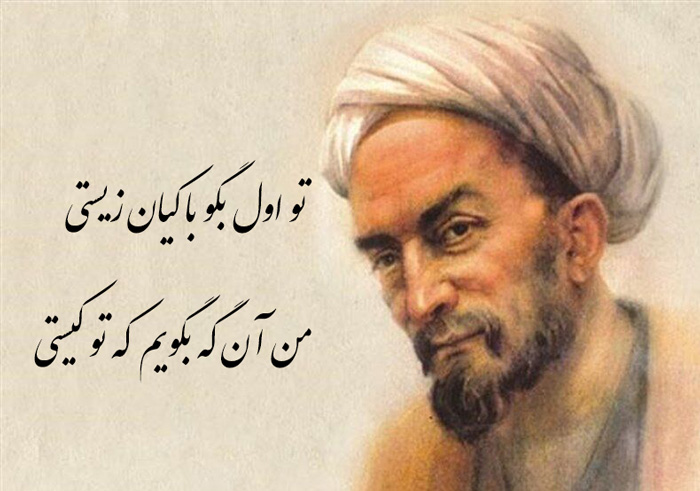
\includegraphics[width=0.6\textwidth]{pic/Saadi.png}
            % \caption{This is the caption of the image.}
            % \label{fig:image1}
            \end{figure}
    \begin{itemize}
        \item First, tell me who you have lived with,
Then, I will tell you who you are.
    \end{itemize}
    
    
    \begin{tikzpicture}[remember picture,overlay]
        \node[anchor=south west, xshift=0.1cm, yshift=0.22cm] at (current page.south west) {
            \scriptsize Figure adapted from https://setare.com
        };
    \end{tikzpicture}
\end{frame}
\begin{frame}{kNN}
    \begin{minipage}{0.5\textwidth}
        \begin{itemize}
            \item K-NN classifier: $k \geq 1$ nearest neighbors
            \begin{itemize}
                \item Label for $x$ predicted by majority voting among its $k-NN$
            \end{itemize}
            \item $k=5$, $x=[x_1, x_2]$
        \end{itemize}
    \end{minipage} %
    \begin{minipage}{0.45\textwidth}
        \begin{figure}[h]
        \centering
        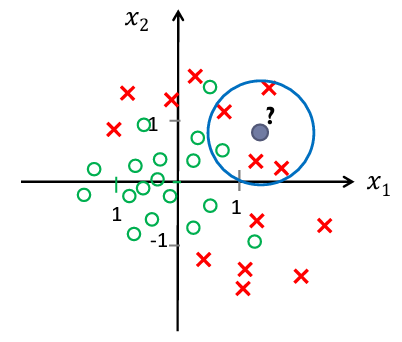
\includegraphics[width=0.8\textwidth]{pic/kE5.png}
        % \caption{This is the caption of the image.}
        % \label{fig:image1}
        \end{figure}
        
        \vfill
    \begin{tikzpicture}[remember picture,overlay]
        \node[anchor=south west, xshift=0.01cm, yshift=0.22cm] at (current page.south west) {
            \scriptsize Figure adapted from M.Soleymani ML slides, Sharif University of Technology
        };
    \end{tikzpicture}
    \end{minipage}
    
    
\end{frame}

%%%%%%%%%%%%%%
\begin{frame}{kNN classifier}
    \begin{itemize}
        \item Given
            \begin{itemize}
                \item Training data $\{(x^{(1)}, y^{(1)}), \dots, (x^{(n)}, y^{(n)})\}$ are simply stored.
            \end{itemize}
        \item To classify $x$:
            \begin{itemize}
                \item Find $k$ nearest training samples to $x$
                \item Out of these $k$ samples, identify the number of samples $k_j$ belonging to class $C_j$ $(j=1, \dots, C)$.
                \item Assign $x$ to the class $C_{j^*}$ where $j^*=\underset{j=1,\dots, c}{\arg\max} \hspace{0.2cm} k_j$
            \end{itemize}
        \item It can be considered as a \textbf{discriminative} method.
    \end{itemize}
\end{frame}
%%%%%%%%%%%%%%%%%%%%%%%%%%%%
\begin{frame}{kNN classifier cont.}
    \begin{itemize}
        \item With \textbf{kNN} we can obtain \textbf{non-linear} decision surfaces unlike the previous methods (linear and logistic regression)
        \item But note that this method could be prone to \textbf{outliers} or \textbf{noisy} data especially if:
        \begin{itemize}
            \item We have \textbf{small dataset}
            \item Our data is \textbf{low-dimensional}
            \item We use a \textbf{small value of} $\mathbf{k}$ (like $k=1$ is only determined by the nearest neighbor and could be misleading in many test cases.
        \end{itemize}
    \end{itemize}
\end{frame}
%%%%%%%%%%%%%%%%%%%%%%%%%%%%%
\begin{frame}{kNN example}
    \begin{itemize}
        \item We want to classify a new document and put it into one of three categories by studying its neighbor samples
    \end{itemize}
    \begin{figure}[h]
            \centering
            
            \includegraphics[width=0.5\textwidth]{pic/kNN?.png}
            % \caption* { \scriptsize [Duda, Hurt, and Strok’s Book]}
            % \label{fig:image1}
            \end{figure}
\end{frame}
%%%%%%%%%%%%%%%%%%%%%%%%%%%%%%%%%%
\begin{frame}{1-Nearest neighbor classifier}
    \begin{figure}[h]
            \centering
            
            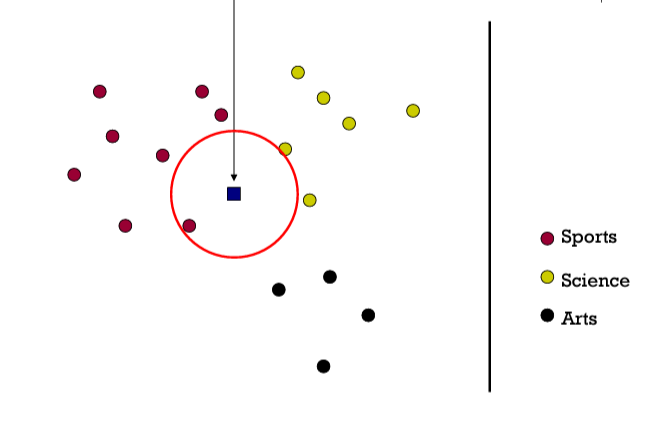
\includegraphics[width=0.7\textwidth]{pic/1NN.png}
            % \caption* { \scriptsize [Duda, Hurt, and Strok’s Book]}
            % \label{fig:image1}
            \end{figure}
\end{frame}
%%%%%%%%%%%%%%%%%%%%%%%%%%%%%
\begin{frame}{2-Nearest neighbor classifier}
    \begin{figure}[h]
            \centering
            
            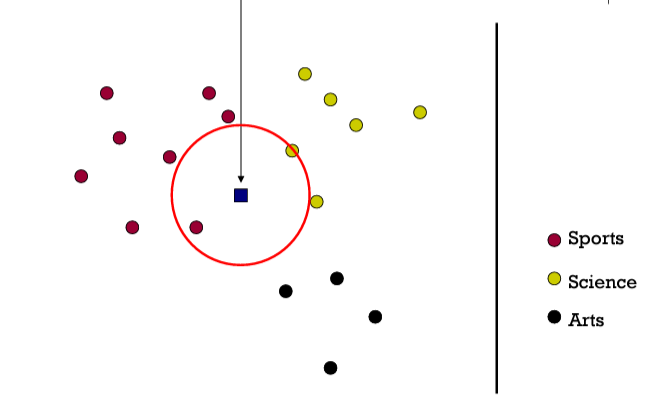
\includegraphics[width=0.7\textwidth]{pic/2NN.png}
            % \caption* { \scriptsize [Duda, Hurt, and Strok’s Book]}
            % \label{fig:image1}
            \end{figure}
\end{frame}
%%%%%%%%%%%%%%%%%%%%%%%%%%%%%
\begin{frame}{3-Nearest neighbor classifier}
    \begin{figure}[h]
            \centering
            
            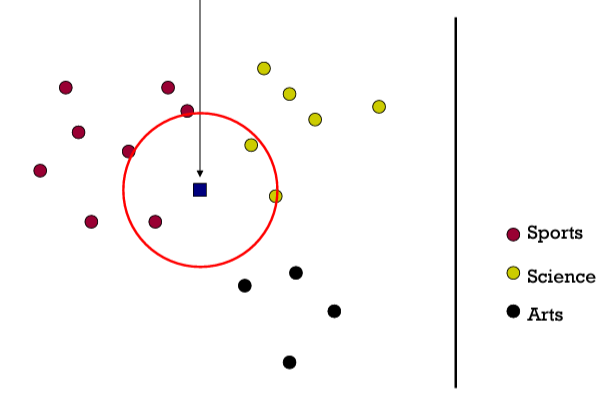
\includegraphics[width=0.7\textwidth]{pic/3NN.png}
            % \caption* { \scriptsize [Duda, Hurt, and Strok’s Book]}
            % \label{fig:image1}
            \end{figure}
\end{frame}
%%%%%%%%%%%%%%%%%%%%%%%%%%%%%
\begin{frame}{5-Nearest neighbor classifier}
    \begin{figure}[h]
            \centering
            
            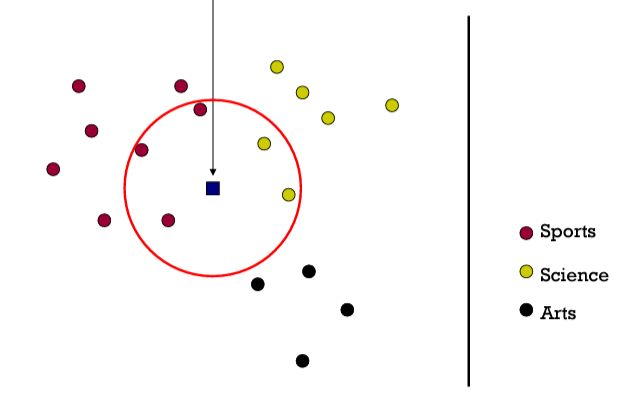
\includegraphics[width=0.7\textwidth]{pic/5NN.png}
            % \caption* { \scriptsize [Duda, Hurt, and Strok’s Book]}
            % \label{fig:image1}
            \end{figure}
    \vfill
    \begin{tikzpicture}[remember picture,overlay]
        \node[anchor=south west, xshift=0.01cm, yshift=0.22cm] at (current page.south west) {
            \scriptsize Figures for this example were adapted from E. Xing, “Theory of classification and nonparametric classifier.” Lecture notes
        };
    \end{tikzpicture}
\end{frame}
%%%%%%%%%%%%%%%%%%%%%%%%%%%%%
\begin{frame}{Voronoi tessellation}

    \begin{itemize}
        \item Voronoi tessellation:
         \begin{itemize}
             \item Each cell consists of all points closer to a given training point than to any other training points
             \item All points in a cell are labeled by the category of the corresponding training point
         \end{itemize}
         
         
    \end{itemize}
    \begin{figure}[h]
            \centering
            
            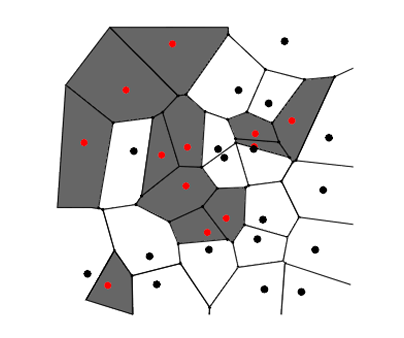
\includegraphics[width=0.35\textwidth]{pic/Voroni.png}
            \caption* { \scriptsize [Duda, Hurt, and Strok’s Book]}
            % \label{fig:image1}
            \end{figure}
\end{frame}
%%%%%%%%%%%%%%%%%%%%%%%%%%%%%
\begin{frame}{Voronoi tessellation}
    \begin{itemize}
        \item 1NN plot is a Voronoi tessellation
    \end{itemize}
    
    \begin{figure}[h]
            \centering
            
            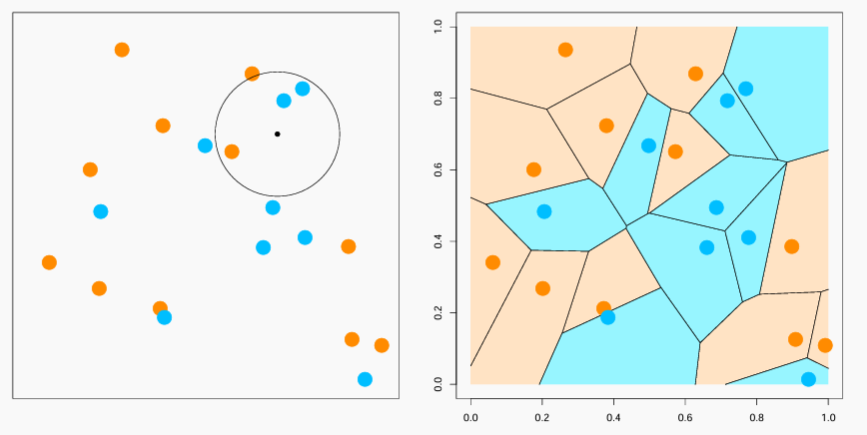
\includegraphics[width=0.8\textwidth]{pic/1NNVoronoi.png}
            % \caption* { \scriptsize [Duda, Hurt, and Strok’s Book]}
            % \label{fig:image1}
            \end{figure}
            
    \vfill
    \begin{tikzpicture}[remember picture,overlay]
        \node[anchor=south west, xshift=0.01cm, yshift=0.22cm] at (current page.south west) {
            \scriptsize Figure adapted from R. Zhu, “Stat 542: Statistical learning - k-nearest neighbor and the bias-variancetrade-off.” Lecture notes.
        };
    \end{tikzpicture}
\end{frame}
%%%%%%%%%%%%%%%%%%%%%%%%%%%%%
\begin{frame}{Effect of k}
    \begin{figure}[h]
            \centering
            
            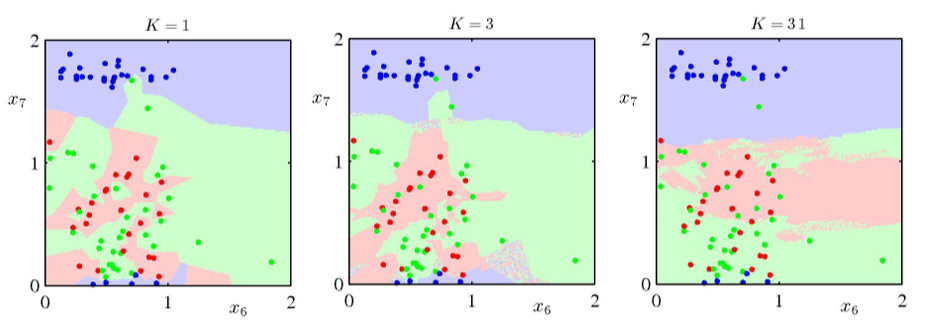
\includegraphics[width=0.9\textwidth]{pic/effectOfK.png}
            \caption* { \scriptsize [Bishop]}
            % \label{fig:image1}
            \end{figure}
\end{frame}
%%%%%%%%%%%%%%%%%%%%%%%%%%%%%%%%%%%%%%%
\begin{frame}{Effect of k cont.}
    \begin{itemize}
        \item compare $k=1$ with $k=15$
    \end{itemize}
    \begin{figure}[h]
            \centering
            
            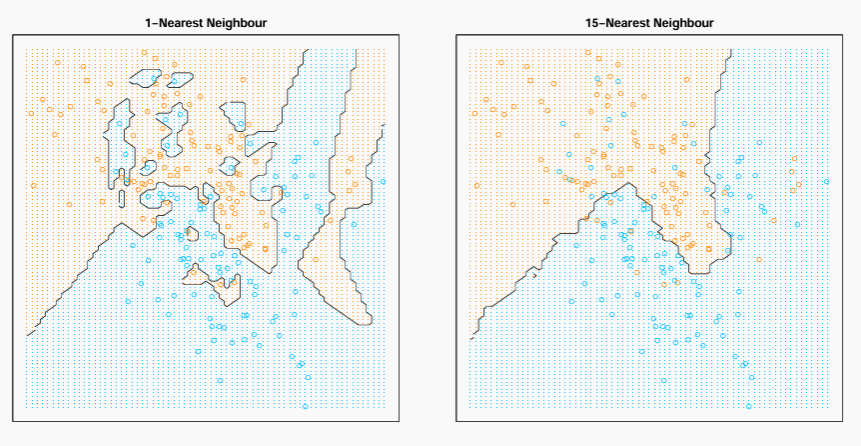
\includegraphics[width=0.7\textwidth]{pic/1vs15.png}
            % \caption* { \scriptsize [Bishop]}
            % \label{fig:image1}
            \end{figure}
    
\end{frame}
%%%%%%%%%%%%%%%%%%%%%%%%%%%%%%%%%%%%%%%
\begin{frame}{Model complexity}
    \begin{itemize}
        \item As we further increase $k$, the model tends to be less complex.
        \item Compare $66NN$ with a linear model that uses only $3$ parameters:
    \end{itemize}
    
    \begin{figure}[h]
            \centering
            
            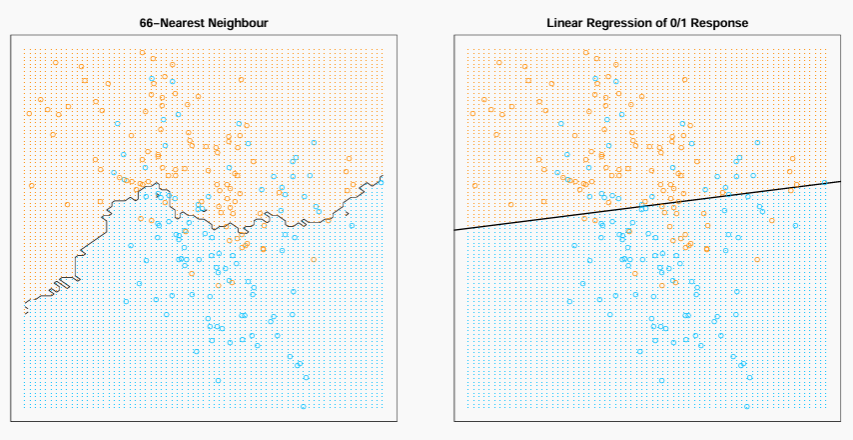
\includegraphics[width=0.7\textwidth]{pic/66vsLin.png}
            % \caption* { \scriptsize [Bishop]}
            % \label{fig:image1}
            \end{figure}
            
    \vfill
    \begin{tikzpicture}[remember picture,overlay]
        \node[anchor=south west, xshift=0.01cm, yshift=0.22cm] at (current page.south west) {
            \scriptsize Figures were adapted from R. Zhu, “Stat 542: Statistical learning - k-nearest neighbor and the bias-variancetrade-off.” Lecture notes.
        };
    \end{tikzpicture}
\end{frame}
%%%%%%%%%%%%%%%%%%%%%%%%%%%%%%%%%%%%%%%%

%%%%%%%%%%%%%%%%%%%%%%%%%%%%%%%%%%%%%%%%
\begin{frame}{Instance-based learner}
    \begin{itemize}
        % \item kNN is an instance-based learner
        \item Main things to construct an instance-based learner:
        \begin{itemize}
            \item A distance metric
            \item Number of nearest neighbors of the test data that we look at
            \item A weighting function (optional)
            \item How to find the output based on neighbors?
        \end{itemize}
    \end{itemize}
\end{frame}

%%%%%%%%%%%%%%%%%%%%%%%%%%%%%%%%%%%%%%%
\begin{frame}{Distance measures}
    \begin{itemize}
        \item Euclidean distance
    \end{itemize}
       \[
          d(x, x') = \sqrt[2]{\|x - x'\|_2^2} = \sqrt[2]{(x_1 - x'_1)^2 + \cdots + (x_d - x'_d)^2}
       \]
    \begin{itemize}
        \item Distance learning methods for this purpose
        \begin{itemize}
            \item Weighted Euclidean distance
             \[
                d_w(x, x') = \sqrt[2]{w_1(x_1 - x'_1)^2 + \cdots + w_d(x_d - x'_d)^2}
             \]
            % \item Mahalanobis distance 
            % \[
            %     d_A(x, x') = \sqrt{(x_1 - x'_1)^TA(x_1-x'_1)}
            % \]
        \end{itemize}
    % \item Other distances:
    %     \begin{itemize}
    %         \item Hamming, angle, L-norm, Mahalanobis distance, ...
    %         % \item $L_p(x, x') = \sqrt[p]{\sum _{i=1}^{d} (x_i - x'_i)^p}$
    %     \end{itemize}
   
    \end{itemize}       
\end{frame}
%%%%%%%%%%%%%%%%%%%%%%%%%%%%%%%%%%%%%%%%%
\begin{frame}{Distance measures cont.}
    \begin{itemize}
         \item Minkowski distance
    \[
    d(x,x') = (\sum _{i=1} ^ n |x_i - x'_i| ^ p ) ^ {\frac{1}{p}}
    \]
        \begin{itemize}
            \item for $p \geq 1$ is a distance metric
            \item As you can see Minkowski distance with $p=2$ is the same as Euclidean distance
            \item Minkowski distance is the same as $L^p$ norm of $(x-x')$
        \end{itemize}
    \item Remember $L^p$ norm from linear algebra:
        \[
            \|x\|_p = \sqrt[p]{(|x_1|^p + \dots + |x_n|^p)}
        \]
        \begin{align*}
            \text{Some famous $L^p$ norms} \begin{cases}
                    \|x\|_1 &= \sum _{i=1}^n |x_i| \\
                    \|x\|_2 &= \sqrt{x_1^2 + \dots + x_n^2} \\
                    \|x\|_{\infty}  &= \max \{|x_1|, |x_2|, \dots, |x_n|\}
                \end{cases}
        \end{align*}
    \end{itemize}
\end{frame}
%%%%%%%%%%%%%%%%%%%%%%%%%%%%%%%%%%%%%%%%%
%%%%%%%%%%%%%%%%%%%%%%%%%%%%%%%%%%%%%%%
\begin{frame}{Distance measures cont.}
    \begin{itemize}
        \item Cosine distance (angle)
    \end{itemize}
    \begin{align*}  
        d(x,x') &= 1 - \text{cosine similarity}(x,x') \\
        \text{Where,} \hspace{0.4cm} \text{cosine similarity}(x,x') &= \frac{x.x'}{\|x\|_2 \|x'\|_2} = \frac{\sum _ {i=1}^d x_i x'_i}{\sqrt{\sum _{i=1}^d x_i^2} \sqrt{\sum _{i=1}^d x'_i^2}}
    \end{align*}
    
    
    \begin{figure}[h]
            \centering
            
            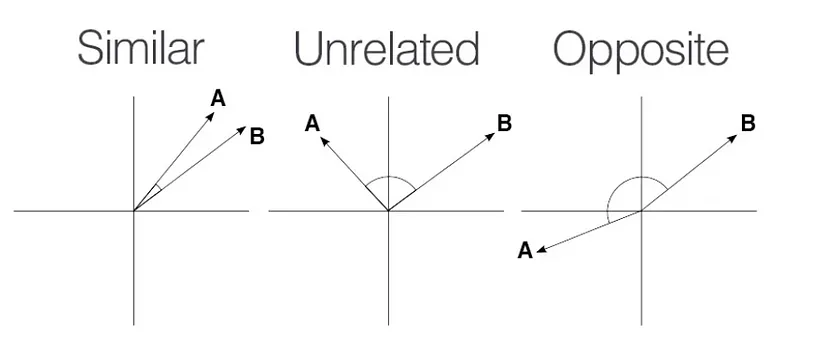
\includegraphics[width=0.5\textwidth]{pic/cosine.png}
            \caption* { \scriptsize Example of angle difference for cosine similarity}
            % \label{fig:image1}
            \end{figure}
    
     \begin{tikzpicture}[remember picture,overlay]
        \node[anchor=south west, xshift=0.1cm, yshift=0.22cm] at (current page.south west) {
            \scriptsize Figure adapted from https://medium.com/@milana.shxanukova15/cosine-distance-and-cosine-similarity-a5da0e4d9ded
        };
    \end{tikzpicture}
\end{frame}
%%%%%%%%%%%%%%%%%%%%%%%%%%%%%%%%%%%%%%%
\begin{frame}{Effect of distance measure}
    \begin{figure}[h]
            \centering
            
            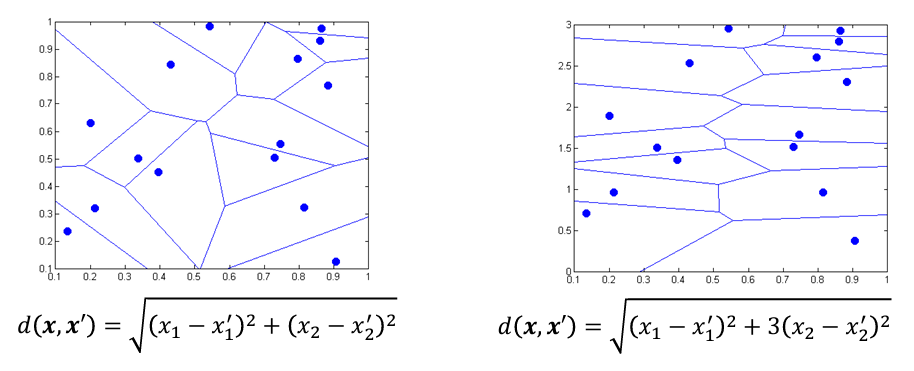
\includegraphics[width=0.9\textwidth]{pic/DistMeasEf.png}
            % \caption* { \scriptsize [}
            % \label{fig:image1}
            \end{figure}
            
    \vfill 
    \begin{tikzpicture}[remember picture,overlay]
        \node[anchor=south west, xshift=0.01cm, yshift=0.15cm] at (current page.south west) {
            \scriptsize Figures adapted from M.Soleymani ML slides, Sharif University of Technology
        };
    \end{tikzpicture}
\end{frame}
%%%%%%%%%%%%%%%%%%%%%%%%%%%%%%%%%%%%%%%%
% \begin{frame}{Probabilistic perspective of kNN}
%     \begin{itemize}
%         \item kNN as a discriminative non-parametric classifier
%           \begin{itemize}
%               \item Non-parametric density estimation for $P(C_j|x)$
%               \item $P(C_j|x) \approx \frac{k_j}{k}$ where $k_j$ shows the number of training samples among $k$ nearest neighbors of $x$ that are labeled $C_j$
%           \end{itemize}
%         \item Bayes decision rule for assigning labels
%     \end{itemize}
% \end{frame}
%%%%%%%%%%%%%%%%%%%%%%%%%%%%%%%%%%
\begin{frame}{kNN regression}
    \begin{itemize}
        \item Let $x'^{(1)}, \dots , x'^{(k)}$ be the $k$ nearest neighbors of $x$ and $y'^{(1)}, \dots, y'^{(k)}$ be their labels.
        \[
            \hat{y} = \frac{1}{k}\sum _{j=1}^k y'^{(j)}
        \]
        \item Some problems of kNN regression for fitting functions:
        \begin{itemize}
            \item Discontinuities in the estimated function
            \item 1NN: noise-fitting problem
            \item kNN ($k>1$) smoothes away noise, but there could be other issues (e.g, flats the ends)
        \end{itemize}
    \end{itemize}
\end{frame}
%%%%%%%%%%%%%%%%%%%%%%%%%%%%%%%%%%%%%%
\begin{frame}{kNN regression cont.}
    \begin{figure}[h]
            \centering
            
            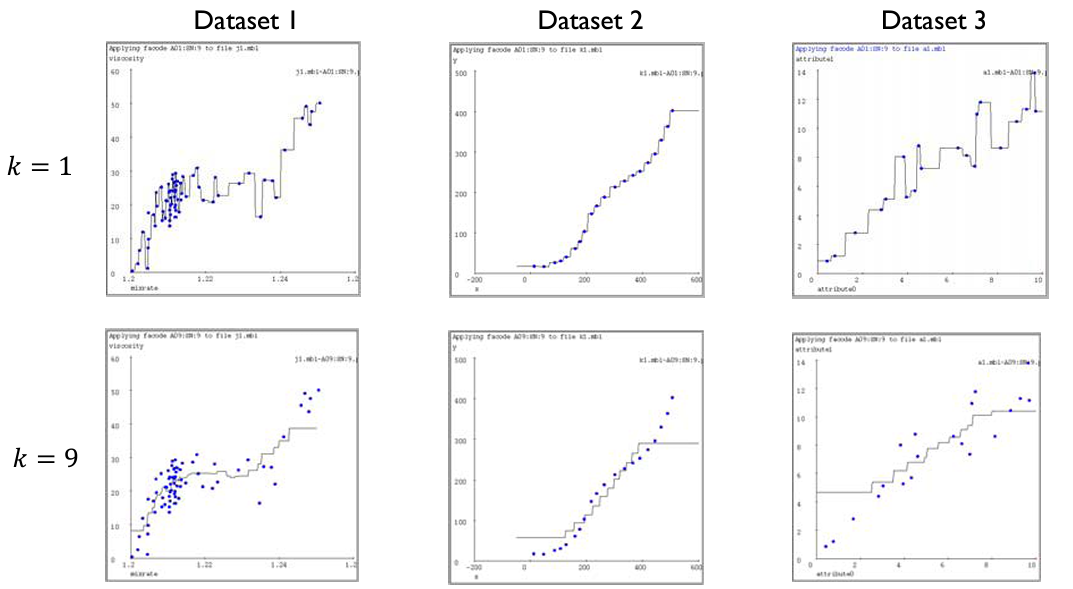
\includegraphics[width=0.75\textwidth]{pic/knnR1.png}
            \caption* { \scriptsize [Figs. have been adopted from Andrew Moore’s tutorial on “Instance-based learning”]}
            % \label{fig:image1}
            \end{figure}
\end{frame}
%%%%%%%%%%%%%%%%%%%%%%%%%%%%%%%%%%%%
\begin{frame}{kNN regression: example}
    \begin{itemize}
        \item Suppose we have a dataset with only 1 feature from uniform $[0, 2\pi]$. The true model is:
        \[Y = 2sin(X) + \epsilon\]
        \item Where $\epsilon$ is the standard normal error.
        \item First we simulate 200 observations, and see the model for $k=1$
    \end{itemize}
    
    \begin{figure}[h]
            \centering
            
            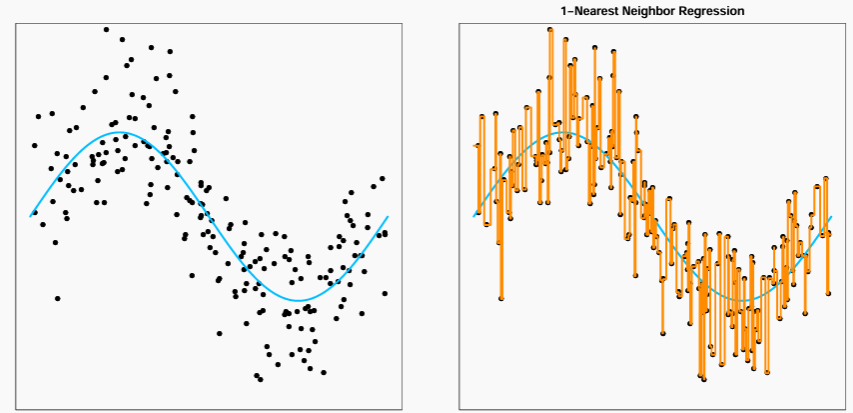
\includegraphics[width=0.6\textwidth]{pic/knnReg1.png}
            % \caption* { \scriptsize [Figs. have been adopted from Andrew Moore’s tutorial on “Instance-based learning”]}
            % \label{fig:image1}
            \end{figure}
    
    % \vfill 
    % \begin{tikzpicture}[remember picture,overlay]
    %     \node[anchor=south west, xshift=0.01cm, yshift=0.15cm] at (current page.south west) {
    %         \scriptsize Figure adapted from R.Zhu, STAT 542, University of Illinois
    %     };
    % \end{tikzpicture}
\end{frame}
%%%%%%%%%%%%%%%%%%%%%%%%%%%%%%%%%%%%
\begin{frame}{kNN regression: example}
    \begin{itemize}
        \item Now for $k=2$ and $k=10$
    \end{itemize}
    
    \begin{figure}[h]
            \centering
            
            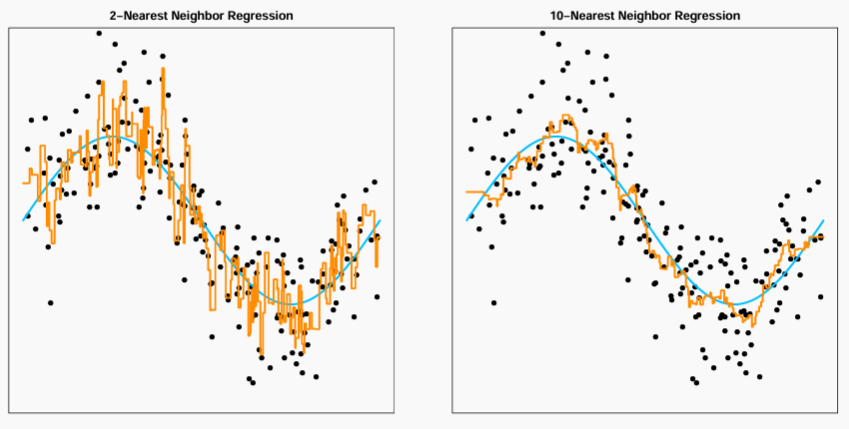
\includegraphics[width=0.8\textwidth]{pic/knnReg2.png}
            % \caption* { \scriptsize [Figs. have been adopted from Andrew Moore’s tutorial on “Instance-based learning”]}
            % \label{fig:image1}
            \end{figure}
            
    % \vfill 
    
    % \begin{tikzpicture}[remember picture,overlay]
    %     \node[anchor=south west, xshift=0.01cm, yshift=0.15cm] at (current page.south west) {
    %         \scriptsize Figure adapted from R.Zhu, STAT 542, University of Illinois
    %     };
    % \end{tikzpicture}
\end{frame}
%%%%%%%%%%%%%%%%%%%%%%%%%%%%%%%%%%%%
\begin{frame}{kNN regression: example}
    \begin{itemize}
        \item As you can see the model becomes smoother as $k$ increases. However, this eventually deviates from the truth if $k$ is too large
    \end{itemize}
    
    \begin{figure}[h]
            \centering
            
            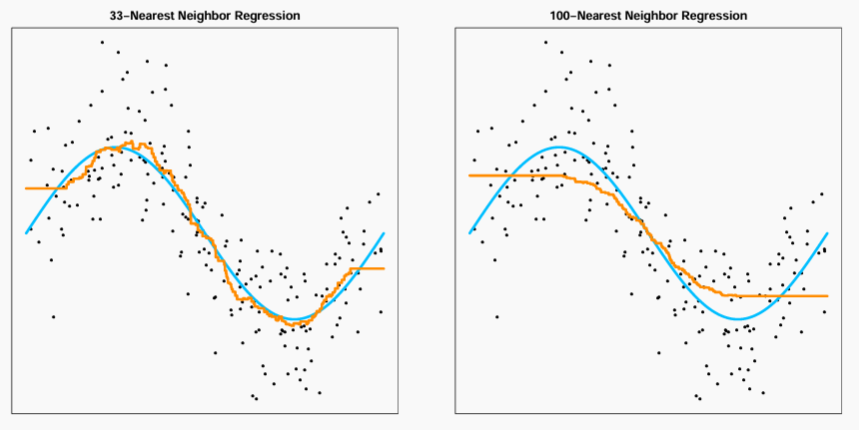
\includegraphics[width=0.8\textwidth]{pic/knnReg3.png}
            % \caption* { \scriptsize [Figs. have been adopted from Andrew Moore’s tutorial on “Instance-based learning”]}
            % \label{fig:image1}
            \end{figure}
    
    \vfill
    \begin{tikzpicture}[remember picture,overlay]
        \node[anchor=south west, xshift=0.01cm, yshift=0.22cm] at (current page.south west) {
            \scriptsize Figures were adapted from R. Zhu, “Stat 542: Statistical learning - k-nearest neighbor and the bias-variancetrade-off.” Lecture notes.
        };
    \end{tikzpicture}
    % \vfill 
    
    % \begin{tikzpicture}[remember picture,overlay]
    %     \node[anchor=south west, xshift=0.01cm, yshift=0.15cm] at (current page.south west) {
    %         \scriptsize Figure adapted from R.Zhu, STAT 542, University of Illinois
    %     };
    % \end{tikzpicture}
\end{frame}
%%%%%%%%%%%%%%%%%%%%%%%%%%%%%%%%%%
\section{Performance metrics}


\begin{frame}{Accuracy in classification problems}
    \begin{itemize}
        \item \textbf{Accuracy} is one of the simplest and most commonly used performance metrics.
        \item It is defined as the ratio of correctly predicted instances to the total instances:
        \[
        \text{Accuracy} = \frac{\text{True Positives} + \text{True Negatives}}{\text{Total Samples}}
        \]
        \item However, accuracy alone can be misleading, especially with imbalanced datasets.
    \end{itemize}
\end{frame}

\begin{frame}{Example: cancer detection problem}
    \begin{itemize}
        \item Imagine a dataset with 1000 patients:
        \begin{itemize}
            \item Only 10 have cancer (\textbf{positive class}).
            \item 990 do not have cancer (\textbf{negative class}).
        \end{itemize}
        \item A classifier predicts that no one has cancer (predicts all as negative).
        \item What will be the accuracy of this model?
    \end{itemize}
\end{frame}

\begin{frame}{Example: cancer detection problem cont.}
    Look at this table for our model which predict negative all the time:
    
    \begin{table}[h!]
        \centering
        \begin{tabular}{@{}lcc@{}}
            \toprule
            & \textbf{Predicted Negative} & \textbf{Predicted Positive} \\ \midrule
            \textbf{Actual Negative} & 990 (TN) & 0 (FP) \\
            \textbf{Actual Positive} & 10 (FN)  & 0 (TP) \\ \bottomrule
        \end{tabular}
        % \caption*{Confusion Matrix for Cancer Detection (All Negative Predictions)}
    \end{table}
    
    \[
    \text{Accuracy} = \frac{990 + 0}{1000} = 99\%
    \]
    
    \textbf{High accuracy}, but the model fails to detect any actual cases of cancer!
\end{frame}


\begin{frame}{Why accuracy can be misleading}
    \begin{itemize}
        \item In highly imbalanced datasets (e.g., cancer detection), the \textbf{minority class} (positive cases) is often underrepresented.
        \item A model that always predicts the majority class can still have high accuracy, but poor real-world performance.
        \item In the cancer detection example, 99\% accuracy sounds good, but the model doesn't detect any actual cancer cases.
        \item We need better metrics to evaluate model performance.
    \end{itemize}
\end{frame}
%%%%%%%%%%%%%%%%%%%%%%%%%%%%%%%%%%%%%%%%%%%%%%%%
\begin{frame}{Performance metrics}
    \begin{itemize}
        \item \textbf{Scenario:}
        \begin{itemize}
            \item An alarm system can either ring or not ring when a thief is present.
            \item Let's define the outcomes:
            \begin{itemize}
                \item \textbf{True Positive (TP)}: Alarm rings (correctly) when a thief is present.
                \item \textbf{True Negative (TN)}: Alarm does not ring (correctly) when no thief is present.
                \item \textbf{False Positive (FP)}: Alarm rings (incorrectly) when no thief is present (a false alarm).
                \item \textbf{False Negative (FN)}: Alarm does not ring (incorrectly) when a thief is present (a missed alarm).
            \end{itemize}
        \end{itemize}
    \end{itemize}
    
    % \begin{table}[h!]
    %     \centering
    %     \begin{tabular}{@{}lcc@{}}
    %         \toprule
    %         & \textbf{Thief Present} & \textbf{No Thief Present} \\ \midrule
    %         \textbf{Alarm Rings} & TP & FP \\
    %         \textbf{Alarm Does Not Ring} & FN & TN \\ \bottomrule
    %     \end{tabular}
    %     % \caption*{Confusion Matrix for Alarm System}
    % \end{table}
    
    \begin{minipage}{0.7\textwidth} % Left side for the table
        \begin{table}[h!]
            \centering
            \begin{tabular}{@{}lcc@{}}
                \toprule
                & \textbf{Thief Present} & \textbf{No Thief Present} \\ \midrule
                \textbf{Alarm Rings} & TP & FP \\
                \textbf{Alarm Does Not Ring} & FN & TN \\ \bottomrule
            \end{tabular}
        \end{table}
        
        
    \end{minipage}\hfill 
    \begin{minipage}{0.2\textwidth} 
        \centering
        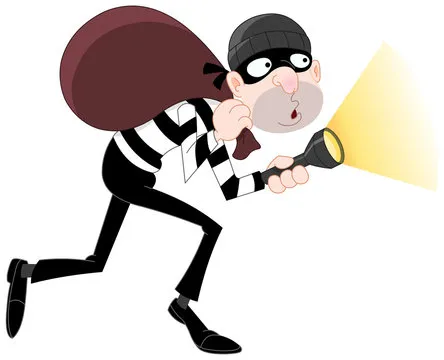
\includegraphics[width=\textwidth]{pic/thief.png} 
        
        \begin{tikzpicture}[remember picture,overlay]
        \node[anchor=south west, xshift=0.1cm, yshift=0.2cm] at (current page.south west) {
            \scriptsize Photo adapted from https://stock.adobe.com/search?k=thief+cartoon
        };
    \end{tikzpicture}
        
    \end{minipage}
    
\end{frame}

\begin{frame}{Performance metrics cont.}
    \begin{itemize}
        \item \textbf{Metrics:}
        \begin{itemize}
            % \item \textbf{Accuracy}:
            % \[
            % \text{Accuracy} = \frac{TP + TN}{TP + TN + FP + FN}
            % \]
            % \textit{Measures the overall correctness of the alarm system. It is the proportion of true results (both true positives and true negatives) among the total cases examined.}
            
            \item \textbf{Sensitivity (Recall)}:
            \[
            \text{Sensitivity} = \frac{TP}{TP + FN}
            \]
            \textit{Indicates the ability of the alarm system to correctly identify a thief. It is the proportion of actual positives (thief present) that are correctly identified.}

            \item \textbf{Specificity}:
            \[
            \text{Specificity} = \frac{TN}{TN + FP}
            \]
            \textit{Measures the ability of the alarm system to correctly identify when no thief is present. It is the proportion of actual negatives that are correctly identified.}

            \item \textbf{Precision}:
            \[
            \text{Precision} = \frac{TP}{TP + FP}
            \]
            \textit{Indicates the accuracy of the alarm when it rings. It is the proportion of times the alarm rang and a thief was indeed present out of all the times the alarm was activated.}
        \end{itemize}
    \end{itemize}
\end{frame}



%%%%%%%%%%%%%%%%%%%%%%%%%%%%%%%%%%%%%%%%%%%%%%%%%
% \begin{frame}{Performance metrics}
    
    
%     \begin{table}[h!]
%     \centering
%     \begin{tabular}{|c|c|c|}
%         \hline
%          & actually in the class & actually not in the  class \\ \hline
%         predicted to be in the class & TP & FP \\ \hline
%         predicted not to be in the class & FN & TN \\ \hline
%         % Row 3, Col 1 & Row 3, Col 2 & Row 3, Col 3 \\ \hline
%     \end{tabular}
%     % \caption{Basic Table}
%     % \label{tab:basic_table}
%     \end{table}
    
    
%     \begin{align*}
%         \text{Precision P } &= \frac{TP}{TP + FP} \\
%         \text{Recall R } &= \frac{TP}{TP + FN} \\
%         \text{Accuracy } &= \frac{TP + TN}{TP + TN + FP + FN}
%     \end{align*}
% \end{frame}
%%%%%%%%%%%%%%%%%%%%%%%%%%%%%%%%%%%%%%%%%%%%%%

%%%%%%%%%%%%%%%%%%%%%%%%%%%%%%%%%%%%%%%%%%%%%%
\begin{frame}{Performance metrics cont.}
    \begin{figure}[h]
            \centering
            
            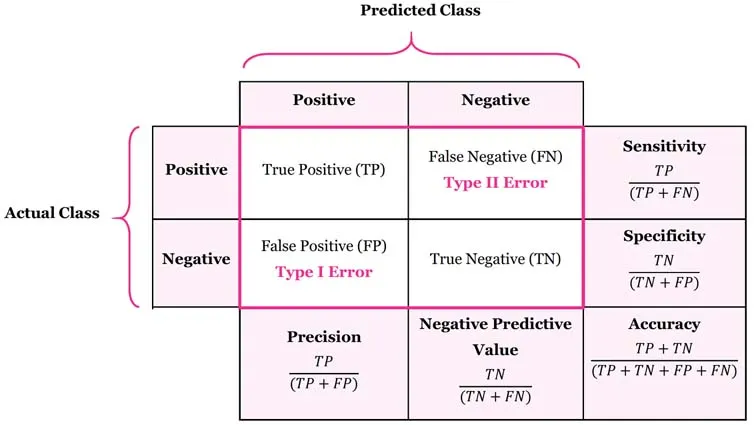
\includegraphics[width=0.8\textwidth]{pic/image.png}
            % \caption* { \scriptsize Figure adapted from }
            % \label{fig:image1}
            \end{figure}
            
    \vfill 
    
    \begin{tikzpicture}[remember picture,overlay]
        \node[anchor=south west, xshift=0.01cm, yshift=0.15cm] at (current page.south west) {
            \scriptsize Figure adapted from https://medium.com

        };
    \end{tikzpicture}
\end{frame}
%%%%%%%%%%%%%%%%%%%%%%%%%%%%%%%%%%%%%%%%%%%%%%
\begin{frame}{A combined measure: F1}
    \begin{itemize}
        \item Combined measure: \textbf{F1 measure}
        \begin{itemize}
            \item allows us to trade off precision and recall
            \item harmonic mean of P and R
        \end{itemize}
    \end{itemize}
    \begin{align*}
        F = \frac{1}{\frac{1}{2P} + \frac{1}{2R}} = \frac{2PR}{P + R}
    \end{align*}
    % \[
    %     \hspace{10cm} \text{You can see: } \beta^2 = \frac{1-\alpha}{\alpha}
    % \]
    
    \begin{itemize}
        \item Harmonic mean of P and R: 
    \end{itemize}
        \begin{align*}
        \frac{1}{F}=\frac{1}{2}(\frac{1}{P}+\frac{1}{R})
    \end{align*}
\end{frame}
%%%%%%%%%%%%%%%%%%%%%%%%%%%%%%%%%%%%%%%%%%%%%
% \begin{frame}{A combined measure: F1 cont.}
%     \begin{itemize}
%         \item People usually use balanced $F$ $(\beta=1 \text{ or } \alpha=\frac{1}{2})$
%     \end{itemize}
%     \begin{align*}
%         F &= F_{\beta=1} \\
%         &\\
%         F &= \frac{2PR}{P + R}
%     \end{align*}
%     \begin{itemize}
%         \item Harmonic mean of P and R: 
%     \end{itemize}
%     \begin{align*}
%         \frac{1}{F}=\frac{1}{2}(\frac{1}{P}+\frac{1}{R})
%     \end{align*}
% \end{frame}
%%%%%%%%%%%%%%%%%%%%%%%%%%%%%%%%%%%%%%%%%%%%%%
\begin{frame}{Precision/recall/F1}
    \begin{itemize}
        \item This website could give you a perfect intuition about precision recall trade-off
        
    \end{itemize}
    \begin{figure}[h]
            \centering
            
            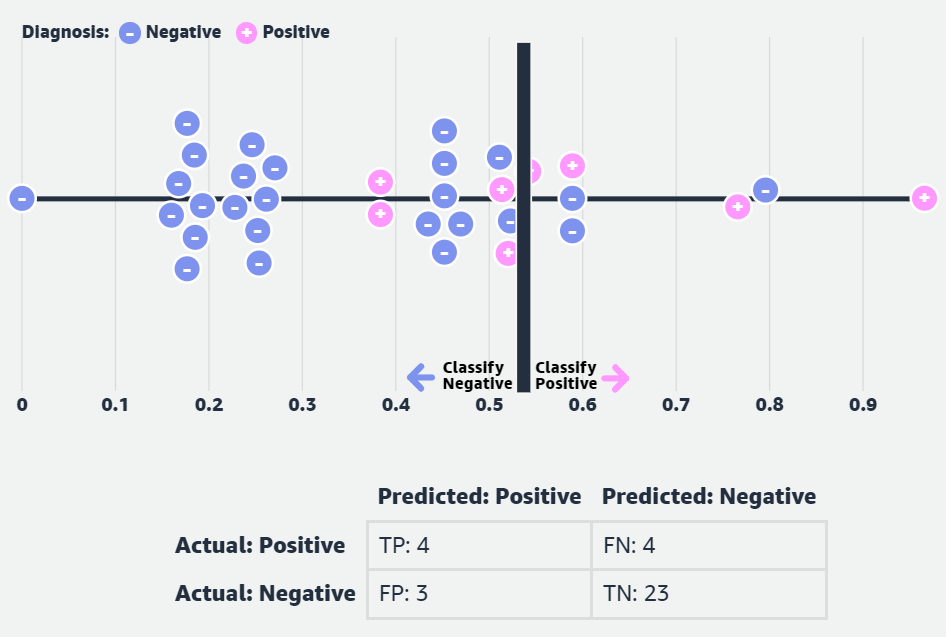
\includegraphics[width=0.5\textwidth]{pic/prRtradeoff.png}
            % \caption* { \scriptsize [}
            % \label{fig:image1}
            \end{figure}
    \begin{itemize}
        \item Link: \href{https://mlu-explain.github.io/precision-recall/}{https://mlu-explain.github.io/precision-recall/}
    \end{itemize}
\end{frame}
%%%%%%%%%%%%%%%%%%%%%%%%%%%%%%%%%%%%%%%%%%%%%%
\begin{frame}{Why harmonic mean?}
    \begin{itemize}
        \item Why don't we use a different mean of P and R as a measure?
        \begin{itemize}
            \item e.g., the arithmetic mean
        \end{itemize}
        \item The simple (arithmetic) mean is $50\%$ for "return true for every thing", which is too high.
        \item Desideratum: Punch really bad performance either on precision or recall
        \begin{itemize}
            \item Taking the minimum achieves this.
            \item F (harmonic mean) is a kind of \textbf{smooth minimum}.
        \end{itemize}
    \end{itemize}
\end{frame}
%%%%%%%%%%%%%%%%%%%%%%%%%%%%%%%%%%%%%%%%%%%%%%
\begin{frame}{F1 and other averages}
    \begin{itemize}
        \item Harmonic mean is a conservative average. We can view the harmonic mean as a kind of soft minimum
    \end{itemize}
    
    \begin{figure}[h]
            \centering
            
            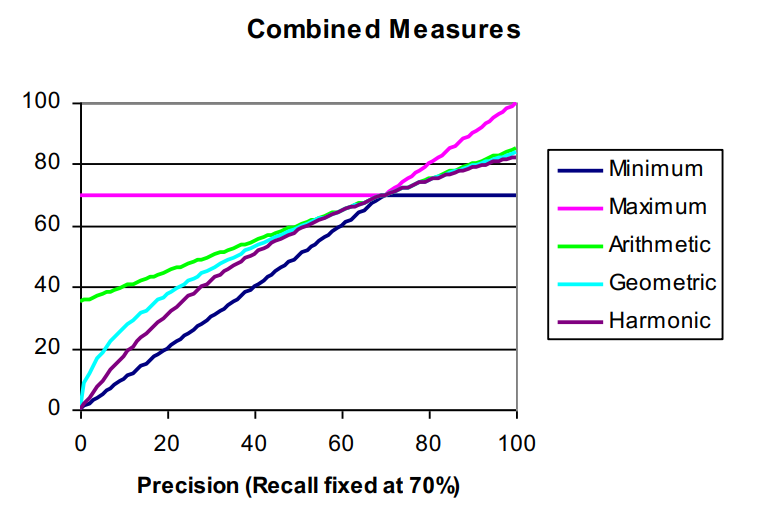
\includegraphics[width=0.58\textwidth]{pic/F1andOthers.png}
            % \caption* { \scriptsize [}
            % \label{fig:image1}
            \end{figure}
    
    \vfill 
    
    \begin{tikzpicture}[remember picture,overlay]
        \node[anchor=south west, xshift=0.01cm, yshift=0.15cm] at (current page.south west) {
            \scriptsize Figure adapted from M.Soleymani ML slides, Sharif University of Technology
        };
    \end{tikzpicture}
\end{frame}
%%%%%%%%%%%%%%%%%%%%%%%%%%%%%%%%%%%%%%%%%%%%%%
% \begin{frame}{A precision-recall curve}
%     \begin{figure}[h]
%             \centering
            
%             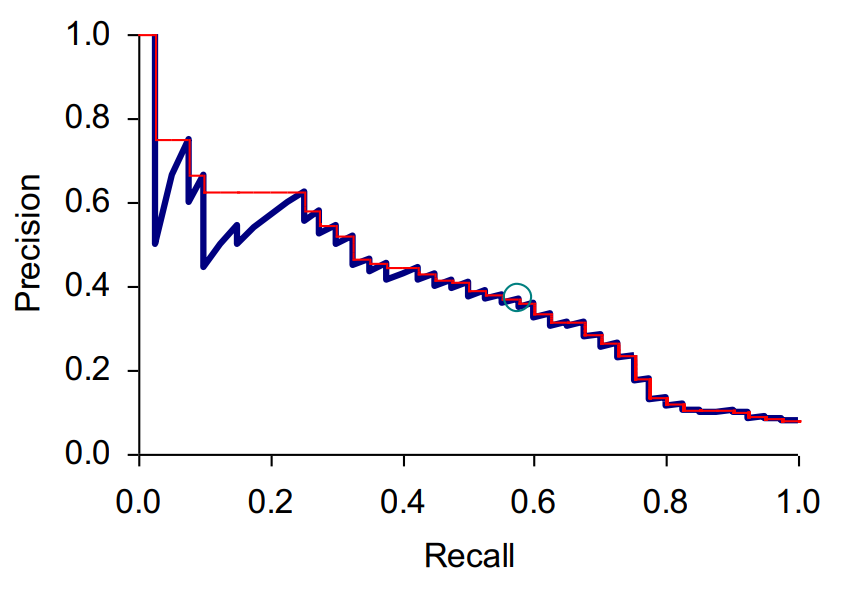
\includegraphics[width=0.68\textwidth]{pic/preReCurv.png}
%             % \caption* { \scriptsize [}
%             % \label{fig:image1}
%             \end{figure}
% \end{frame}
%%%%%%%%%%%%%%%%%%%%%%%%%%%%%%

%%%%%%%%%%%%%%%%%%%%%%%%%%%%
\begin{frame}{Confusion matrix}
    \begin{itemize}
        \item The \textbf{confusion matrix} is a \textbf{table} used to evaluate the performance of a classification model.
        \item It compares the \textbf{actual values (true labels)} with the \textbf{predicted values} from the model.
        \item Each \textbf{row} of the matrix represents the \textbf{actual class}, while each \textbf{column} represents the \textbf{predicted class}.
        \item It helps us understand not just how often the model is correct, but also \textbf{where it makes mistakes}.
    \end{itemize}
    
    % \vfill
    % \centering
    % \includegraphics[width=0.5\textwidth]{confusion_matrix_image.png}
    % % Add an illustrative image of a confusion matrix
\end{frame}


%%%%%%
\begin{frame}{Confusion matrix cont.}
    \begin{itemize}
        \item Let's consider an image classification task where we classify images into three categories: **Cat**, **Dog**, and **Horse**.
        \item After training the model, we evaluate its predictions against the actual labels.
    \end{itemize}
    
    \vfill
    \centering
    \begin{tabular}{|c|c|c|c|}
    \hline
    & \textbf{Predicted Cat} & \textbf{Predicted Dog} & \textbf{Predicted Horse} \\
    \hline
    \textbf{Actual Cat} & True Positive (TP) & False Negative (FN) & False Negative (FN) \\
    \hline
    \textbf{Actual Dog} & False Negative (FN) & True Positive (TP) & False Negative (FN) \\
    \hline
    \textbf{Actual Horse} & False Negative (FN) & False Negative (FN) & True Positive (TP) \\
    \hline
    \end{tabular}
\end{frame}

%%%%%%%
\begin{frame}{Confusion matrix cont.}
    \begin{minipage}{0.4\textwidth}
        \begin{itemize}
            \item Here is an example confusion matrix for a model that classifies images of cats, dogs, and horses:
            \item We can see that the model classified 8 images of cats correctly, but it classified 1 cat as a dog and 1 cat as a horse (False Negatives).
            \item Similarly, it made 2 mistakes when predicting dogs and horses.
        \end{itemize}
    \end{minipage}
    \hfill
    \begin{minipage}{0.55\textwidth}
        \begin{figure}[h]
            \centering
            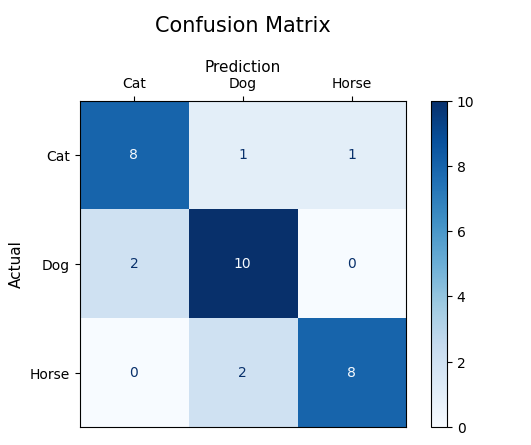
\includegraphics[width=1\textwidth]{pic/cmCatDogHorse.png}
            \caption* {\scriptsize Figure adapted from https://www.geeksforgeek}
        \end{figure}
    \end{minipage}
\end{frame}


%%%%%%%%%%%%%%%%%%%%%%%%%%%%%%
% \begin{frame}{Confusion matrix}
%     \begin{itemize}
%         \item This  $(i,j)$ entry means $53$ of the samples actually in class $i$ were put in class $j$ by the classifier:
%     \end{itemize}
%     \begin{figure}[h]
%             \centering
            
%             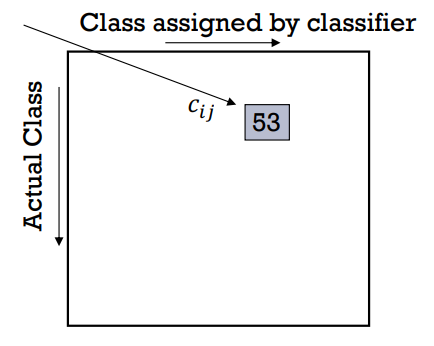
\includegraphics[width=0.4\textwidth]{pic/cmatrix.png}
%             % \caption* { \scriptsize [}
%             % \label{fig:image1}
%             \end{figure}
%     \begin{itemize}
%         \item In a perfect classification, only the diagonal has non-zero entries
%     \end{itemize}
% \end{frame}
%%%%%%%%%%%%%%%%%%%%%%%%%%%%%%%%%%%%%%%%%%%
\begin{frame}{Per class evaluation measures}
    \begin{itemize}
        \item \textbf{Definition:} For our \textbf{confusion matrix} $\mathbf{C}$, each \textbf{element} $\mathbf{C_{ij}}$ denotes the number of samples actually in class $i$ that were put in class $j$ by our classifier.
        \begin{itemize}
            \item Now we could rewrite our performance metrics with confusion matrix view
        \end{itemize}
        \noindent\hrulefill 
        \item Recall: Fraction of the samples in class $i$ classified correctly:
        \[
          \frac{C_{ii}}{\sum _{j} C_{ij}}    
        \]
        \item Precision: Fraction of the samples assigned class $i$ that are actually about class $i$:
        \[
          \frac{C_{ii}}{\sum _{j} C_{ji}}
        \]
        \item Accuracy: Fraction of the samples classified correctly:
        \[
          \frac{\sum _i {C_{ii}}}{\sum _j \sum _i C_{ij}}
        \]
    \end{itemize}
    
\end{frame}
%%%%%%%%%%%%%%%%%%%%%%%%%%%%
\begin{frame}{Averaging: macro vs. micro}
    \begin{itemize}
        \item We now have an evaluation measure (F1) for one class.
        \item But we also want a single number that shows \textcolor{deepred}{aggregate performance} over all classes
    \end{itemize}
\end{frame}
%%%%%%%%%%%%%%%%%%%%%%%%%%%%
\begin{frame}{Micro- vs. Macro-Averaging}
    \begin{itemize}
        \item If we have more than one class, how do we combine
multiple performance measures into one quantity?
        \item \textcolor{deepred}{Macroaveraging}: Compute performance for each class, then average
        \begin{itemize}
            \item Compute F1 for each of the $C$ classes
            \item Average these $C$ numbers
        \end{itemize}
        \item \textcolor{deepred}{Microaveraging}: Collect decisions for all classes, aggregate them and then compute measure.
        \begin{itemize}
            \item Compute TP, FP, FN for each of the $C$ classes.
            \item Sum these $C$ numbers(e.g, all TP to get aggregate TP)
            \item Compute F1 for aggregate TP, FP, FN
        \end{itemize}
    \end{itemize}
\end{frame}
%%%%%%%%%%%%%%%%%%%%%%%%%%%%
\begin{frame}{Micro- vs. Macro-Averaging: example}
    \begin{figure}[h]
            \centering
            
            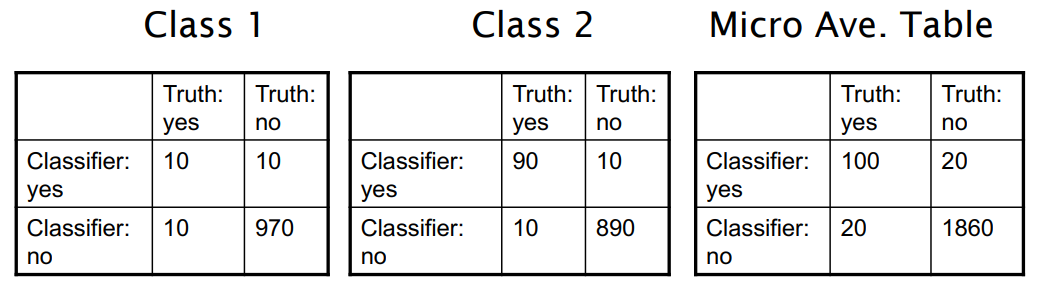
\includegraphics[width=0.8\textwidth]{pic/MicroVsMacro.png}
            % \caption* { \scriptsize [}
            % \label{fig:image1}
            \end{figure}
            
    \begin{itemize}
        \item Macroaveraged precision: $(0.5 + 0.9)/2 = 0.7$
        \item Microaveraged precision: $100/120 = 0.83$
        \item Microaveraged score is dominated by score on common classes
    \end{itemize}
\end{frame}
%%%%%%%%%%%%%%%%%%%%%%%%%%%
% \begin{frame}{Imbalanced classification}
%     \begin{itemize}
%         \item Accuracy is not a proper criteria
%         \item Micro-F1 for multi-class classification is equal to accuracy
%         \item Macro-F1 is more suitable for this purpose
%     \end{itemize}
% \end{frame}
%%%%%%%%%%%%%%%%%%%%%%%%%%%%%
\begin{frame}{AUC-ROC}
    \begin{itemize}
        \item Area Under the Receiver Operating Characteristic Curve
        \begin{itemize}
            \item ROC (Receiver Operating Characteristic) is a graphical representation of the performance of a binary classification model.
            \item It plots the true positive rate (TPR) against the false positive rate (FPR) at different classification thresholds.
        \end{itemize}
        
    \end{itemize}
    
    \begin{figure}[h]
            \centering
            
            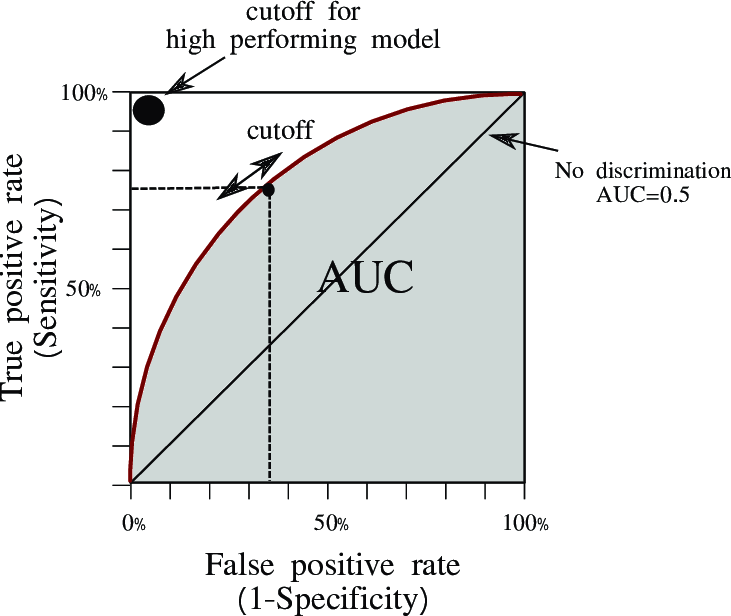
\includegraphics[width=0.4\textwidth]{pic/AUC.png}
            % \caption* { \scriptsize [}
            % \label{fig:image1}
            \end{figure}
    
    \vfill 
    
    \begin{tikzpicture}[remember picture,overlay]
        \node[anchor=south west, xshift=0.01cm, yshift=0.15cm] at (current page.south west) {
            \scriptsize Figure adapted from https://www.researchgate.net/figure/ROC-curves-and-area-under-curve-AUC_fig2_351506473

        };
    \end{tikzpicture}
    
\end{frame}

%%%%%%%%%%%%%%%%%%%%%%%%%%%
\begin{frame}{AUC-ROC cont.}
    \begin{itemize}
        \item A high AUC score indicates that the model has good discrimination ability, i.e., it can effectively differentiate between positive and negative instances at different classification thresholds.
        \item Conversely, a lower AUC-ROC score suggests that the model struggles to differentiate between the two classes.
        \item AUC ranges from 0 to 1, with 0.5 indicating random guessing and 1 indicating a perfect classifier.


    \end{itemize}
\end{frame}
%%%%%%%%%%%%%%%%%%%%%%%%%%%%

\section{Cross Validation}

\begin{frame}{Model Selection via Cross Validation}
    \begin{itemize}
        \item \textbf{Cross-Validation}
        \medskip
        \begin{itemize}\itemsep1em
            \item \justifying \textbf{Purpose}:
            Technique for evaluating how well a model generalizes to unseen data.
            \item \justifying \textbf{How It Works}:
            Split data into $k$ folds; train on $k-1$ folds and validate on the remaining fold.
            \item \justifying \textbf{Repeat Process}:
            Repeat $k$ times, rotating the test fold each time. Average of all scores is the final score of the model.
            \item \justifying Cross-validation
            reduces overfitting and provides a more reliable estimation of model performance.
            \item Note that the model must be \textbf{retrained} at each iteration to avoid reusing a model that has already seen the test data, ensuring unbiased evaluation.
        \end{itemize}
    \end{itemize}
\end{frame}


\begin{frame}{K-Fold Cross Validation}
    \begin{figure}
        \centering
        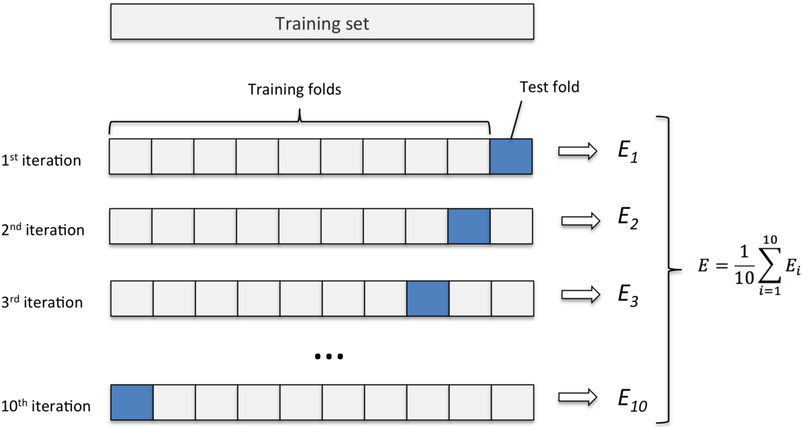
\includegraphics[width=.8\textwidth]{pic/Figure_28.png}
    \end{figure}
    \vfill
    \begin{tikzpicture}[remember picture,overlay]
        \node[anchor=south west, xshift=0.1cm, yshift=0.22cm] at (current page.south west) {
            \scriptsize Figure adapted from Introduction to Support Vector Machines and Kernel Methods, J.M. Ashfaque.
        };
    \end{tikzpicture}
\end{frame}


\begin{frame}{Leave-One-Out Cross-Validation (LOOCV)}
    \begin{itemize}
        \item \textbf{Leave-One-Out Cross-Validation (LOOCV)}
            \medskip
            \begin{itemize}\itemsep1em
            \item \justifying \textbf{How It Works}:
            Uses a single data point as the validation set ($k$ = 1) and the rest as the training set. Repeat for all data points.
            \item \textbf{Properties:}
            \smallskip
            \begin{itemize}\itemsep.5em
                \item \textbf{No Data Wastage}:
                Every data point is used for both training and validation.
                \item \textbf{High Variance, Low Bias}.
                \item \justifying \textbf{Computationally Expensive}: 
                Requires training the model $N$ times for $N$ data points, making it slow for large datasets.
                \item \textbf{Best for small datasets}.
            \end{itemize}
        \end{itemize}
    \end{itemize}
\end{frame}

\begin{frame}{Cross-Validation for Better Generalization}
    \begin{itemize}
        \item Cross-validation is one of the methods used to find the optimal model degree and regularization parameter, ensuring better generalization by minimizing validation error and balancing model complexity.
    \end{itemize}
    \begin{figure}
        \centering
        \begin{minipage}{0.48\linewidth}
            \centering
            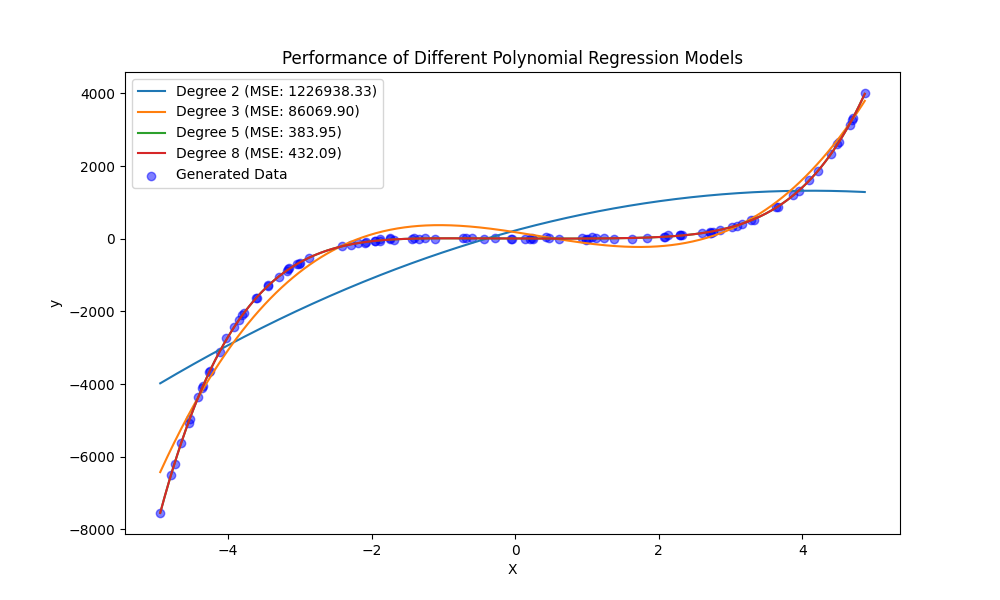
\includegraphics[width=\linewidth]{pic/Figure_16.png}
        \end{minipage}
        \hfill
        \begin{minipage}{0.48\linewidth}
            \centering
            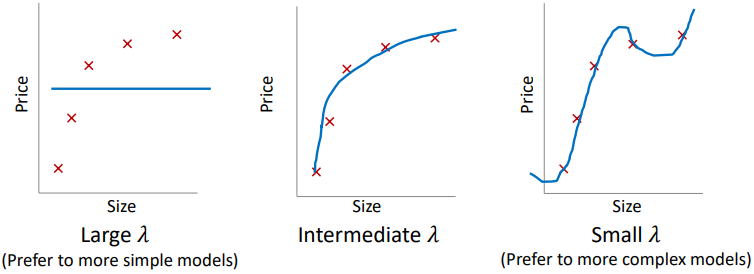
\includegraphics[width=\linewidth]{pic/Figure_29.png}
        \end{minipage}
    \end{figure}
    \begin{tikzpicture}[remember picture,overlay]
        \node[anchor=south west, xshift=0.1cm, yshift=0.22cm] at (current page.south west) {
            \scriptsize Figure on the right adapted from slides of F.Salehi, Machine Learning course, Sharif University of Technology.
        };
    \end{tikzpicture}
\end{frame}



\begin{frame}{Cross-Validation for Evaluating Model Performance}
    \begin{itemize}\itemsep1.2em
        \item Metrics like accuracy, precision, recall, and F1 score are assessed across different folds.
        \item Averaging these scores gives a reliable estimate of performance and stability.
        \item Ensures the model is effective before final testing and use on the test dataset.
        \item \justifying For example, high variance in cross-validation metrics means the model's performance is inconsistent, likely overfitting to specific data subsets.
    \end{itemize}
\end{frame}

%%%%%%%%%%%%%%%%%%%%%%%%%%%%%%%%%
\section{References}

\begin{frame}{Contributions}
\begin{itemize}
\item \textbf{These slides are authored by:}
\medskip
\begin{itemize}
    \setlength{\itemsep}{10pt} % Adjust the value to control the spacing
    \item \href{https://github.com/Danial-Gharib}{Danial Gharib}
    \item \href{https://github.com/Mahan-Bayhaghi}{Mahan Bayhaghi}
    \item \href{https://github.com/jefri021}{Erfan Jafari}
\end{itemize}
\end{itemize}

\end{frame}

\begin{frame}[allowframebreaks]
    \bibliography{ref}
    \bibliographystyle{ieeetr}
    \nocite{*}
\end{frame}

\end{document}